\documentclass[12pt,letterpaper]{article}
\usepackage[utf8]{inputenc}
\usepackage[spanish,es-noshorthands]{babel}
\usepackage{amsmath,amssymb}
\usepackage{graphicx}
\usepackage{tikz}
\usetikzlibrary{arrows.meta}
\usepackage[margin=2.2cm]{geometry}
\usepackage{enumerate}
\setlength{\parindent}{0pt}

% Figura 3b: lazo rectangular en el plano xy (perspectiva oblicua)
% #1 = largo del lado 12 (en el dibujo), #2 = largo del lado 23, #3 = etiqueta a, #4 = etiqueta b
% #5 = punta de flecha: -> (antihorario, 1->2->3->4) o <- (horario, 1->4->3->2)
\newcommand{\figlazo}[5]{%
\begin{tikzpicture}[>=Stealth, line width=0.9pt,
    x={(1cm,0cm)}, y={(0.62cm,0.46cm)}, z={(0cm,1cm)}]
    % ejes (x horizontal, y hacia el fondo, z vertical)
    \draw[->] (0,0,0) -- (#1+1.2,0,0) node[right]{$x$};
    \draw[->] (0,0,0) -- (0,#2+1.3,0) node[above right]{$y$};
    \draw[->] (0,0,0) -- (0,0,2.6) node[above]{$z$};
    % lazo 1-2-3-4
    \draw[line width=1.6pt] (0,0,0) -- (#1,0,0) -- (#1,#2,0) -- (0,#2,0) -- cycle;
    \fill (0,0,0) circle (1.6pt); \fill (#1,0,0) circle (1.6pt);
    \fill (#1,#2,0) circle (1.6pt); \fill (0,#2,0) circle (1.6pt);
    \node[below left]  at (0,0,0)    {$1$};
    \node[below right] at (#1,0,0)   {$2$};
    \node[right]       at (#1,#2,0)  {$3$};
    \node[above left]  at (0,#2,0)   {$4$};
    % sentido de la corriente
    \draw[#5,red,line width=1.3pt] (0.35*#1,0,0) -- (0.65*#1,0,0);
    \draw[#5,red,line width=1.3pt] (#1,0.35*#2,0) -- (#1,0.65*#2,0);
    \draw[#5,red,line width=1.3pt] (0.65*#1,#2,0) -- (0.35*#1,#2,0);
    \draw[#5,red,line width=1.3pt] (0,0.65*#2,0) -- (0,0.35*#2,0);
    \node[red] at (0.5*#1,0.5*#2,0) {$I$};
    % cotas de los lados
    \node[below] at (0.5*#1,-0.1,0) {$#3$};
    \node[right] at (#1+0.12,0.5*#2,0) {$#4$};
\end{tikzpicture}}

\begin{document}

%======================================================================
\begin{center}
    {\Large\textbf{Certamen 3 -- Problema 3 -- FORMA A}}
\end{center}
\medskip

\textbf{3a)} Considere una carga puntual $q = -5\ [\mu\text{C}]$ que se mueve con rapidez
$v = 4\times10^{5}\ [\text{m/s}]$ en una regi\'on del espacio donde hay un campo magn\'etico de
intensidad $B = 0{,}02\ [\text{T}]$. Si las direcciones de la velocidad de la carga y del campo
magn\'etico se indican en la Fig.~3a, determine la fuerza magn\'etica $\vec{F}_m$ ejercida sobre la
carga puntual.

\begin{center}
    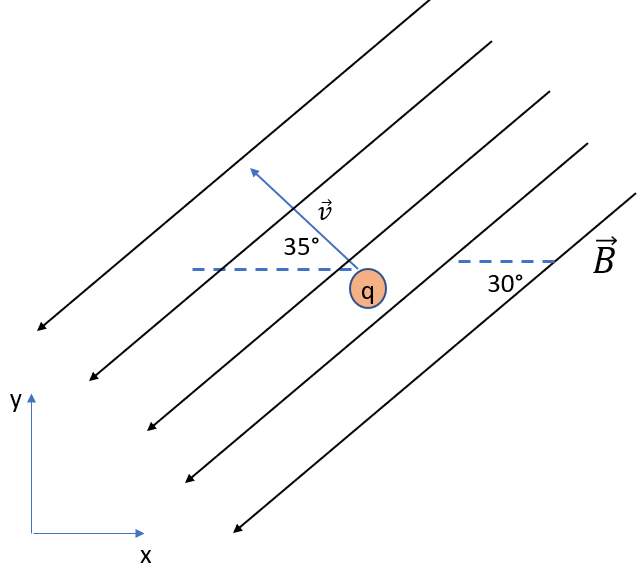
\includegraphics[width=0.48\textwidth]{fig3a.png}\\[2pt]
    Figura 3a
\end{center}

\textbf{3b)} Considere un lazo de corriente de forma rectangular, de lados $a = 8\ [\text{cm}]$ y
$b = 5\ [\text{cm}]$, que se encuentra sobre el plano $xy$, como muestra la Fig.~3b. Por el lazo
circula una corriente $I = 2{,}5\ [\text{A}]$ en sentido antihorario y en la
regi\'on hay un campo magn\'etico $\vec{B} = 0{,}8\,\hat{\jmath} - 0{,}3\,\hat{k}\ [\text{T}]$.
Determine:
\begin{enumerate}[(i)]
    \item La fuerza magn\'etica $\vec{F}_m$ sobre los tramos $12$ y $23$ del lazo de corriente.
    \item El momento magn\'etico $\vec{\mu}$ del lazo de corriente.
    \item El torque magn\'etico $\vec{\tau}$ que ejerce el campo sobre la espira.
\end{enumerate}

\begin{center}
    \figlazo{4.8}{3.0}{a}{b}{->}\\[2pt]
    Figura 3b
\end{center}

\newpage

%======================================================================
\begin{center}
    {\Large\textbf{Certamen 3 -- Problema 3 -- FORMA B}}
\end{center}
\medskip

\textbf{3a)} Considere una carga puntual $q = -4\ [\mu\text{C}]$ que se mueve con rapidez
$v = 3\times10^{5}\ [\text{m/s}]$ en una regi\'on del espacio donde hay un campo magn\'etico de
intensidad $B = 0{,}05\ [\text{T}]$. Si las direcciones de la velocidad de la carga y del campo
magn\'etico se indican en la Fig.~3a, determine la fuerza magn\'etica $\vec{F}_m$ ejercida sobre la
carga puntual.

\begin{center}
    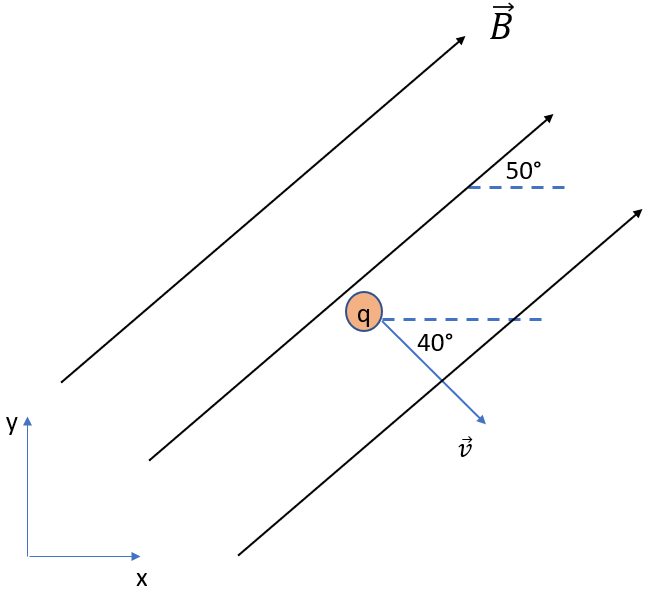
\includegraphics[width=0.48\textwidth]{fig3a_2.png}\\[2pt]
    Figura 3a
\end{center}

\textbf{3b)} Considere un lazo de corriente de forma rectangular, de lados $a = 10\ [\text{cm}]$ y
$b = 6\ [\text{cm}]$, que se encuentra sobre el plano $xy$, como muestra la Fig.~3b. Por el lazo
circula una corriente $I = 1{,}5\ [\text{A}]$ en sentido horario y en la
regi\'on hay un campo magn\'etico $\vec{B} = 0{,}5\,\hat{\imath} - 0{,}4\,\hat{k}\ [\text{T}]$.
Determine:
\begin{enumerate}[(i)]
    \item La fuerza magn\'etica $\vec{F}_m$ sobre los tramos $12$ y $23$ del lazo de corriente.
    \item El momento magn\'etico $\vec{\mu}$ del lazo de corriente.
    \item El torque magn\'etico $\vec{\tau}$ que ejerce el campo sobre la espira.
\end{enumerate}

\begin{center}
    \figlazo{5.0}{3.0}{a}{b}{<-}\\[2pt]
    Figura 3b
\end{center}

\end{document}
